\documentclass{beamer}
\newif\ifplacelogo
\placelogotrue
\mode<presentation>{\usetheme{Boadilla2}}

\usepackage{geometry}
\usepackage{color}
\usepackage{graphicx}

\usepackage[T1]{fontenc}
\usepackage{fontspec}
\setmainfont{CenturyGothic}
\setsansfont{CenturyGothic}

\AtBeginSection[]{\frame{\tableofcontents[currentsection]}}

\definecolor{myturquoise}{RGB}{0,176,176}
\definecolor{mylightturquoise}{RGB}{54,216,216}


\begin{document}


\setlength{\unitlength}{1mm}
\title{DS Visualisation and Analysis}
\author[Abbey Waldron]{Abbey Waldron}
\date[September 25th, 2015]{}




\setbeamertemplate{navigation symbols}{}

{
\placelogofalse
\begin{frame}
  \titlepage
\end{frame}
}



\begin{frame}{This Week - Fitting, Interpolation and Prediction}

\begin{enumerate}
\item Show last week's work to the class
\item Fitting
\item Interpolation and Prediction
\item Start work on problems
\end{enumerate}

\end{frame}



\begin{frame}{Random Student Generator}

\end{frame}



\begin{frame}{Correlations}

\end{frame}


\begin{frame}{Functions Q1}
\begin{center}
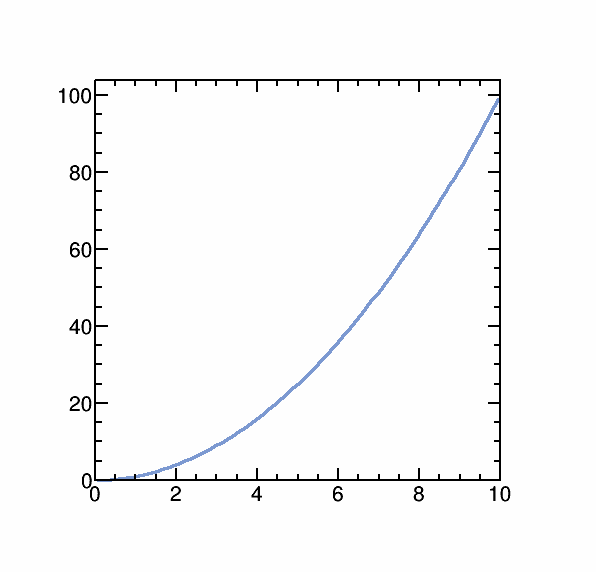
\includegraphics[scale=0.3]{pics/wk3/q1.png}
\end{center}
\end{frame}

\begin{frame}{Q1 Solution}

\[
f(x) = x^{2}
\]

\end{frame}


\begin{frame}{Functions Q2}
\begin{center}
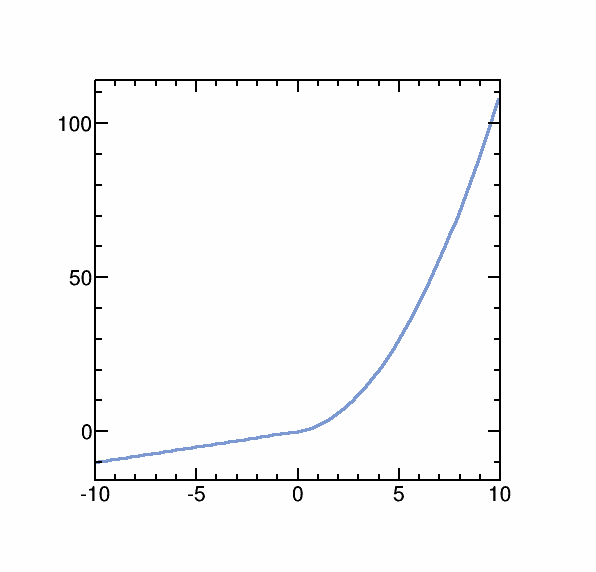
\includegraphics[scale=0.3]{pics/wk3/q2.png}
\end{center}
\end{frame}


\begin{frame}{Q2 Solution}

\[
f(x) = x + 0.5x^{2}(1+\textrm{erf}(x))
\]

\end{frame}

\begin{frame}{Functions Q3}
\begin{center}
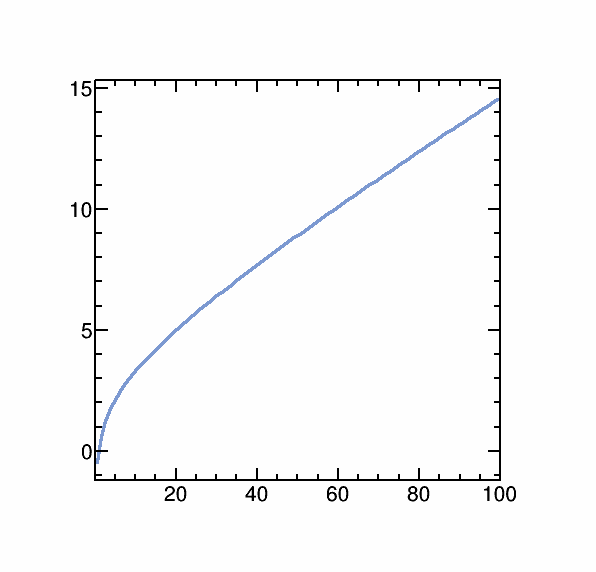
\includegraphics[scale=0.3]{pics/wk3/q3.png}
\end{center}
\end{frame}

\begin{frame}{Q3 Solution}


\[
f(x) = \log{x} + 0.1x
\]

\end{frame}

\begin{frame}{Functions Q4}
\begin{center}
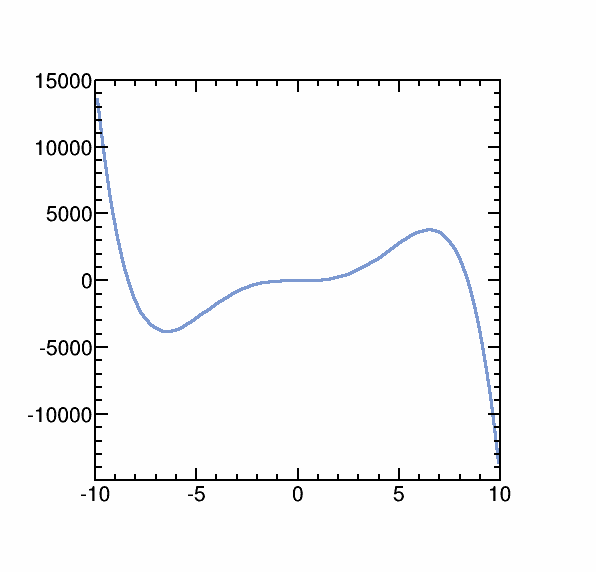
\includegraphics[scale=0.3]{pics/wk3/q4.png}
\end{center}
\end{frame}

\begin{frame}{Q4 Solution}

\[
f(x) = 35x^{3} - 0.5x^{5} 
\]

\end{frame}

\begin{frame}{Functions Q5}
\begin{center}
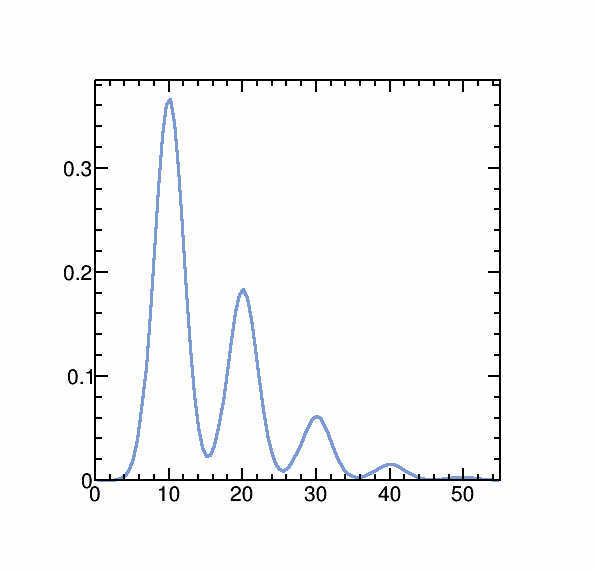
\includegraphics[scale=0.3]{pics/wk3/q5.png}
\end{center}
\end{frame}


\begin{frame}{Q5 Solution}

$\mu = 10$, $\sigma = 2$, $\lambda = 1$

\[
f(x) = \sum_{i=1}^{n}\texttt{dnorm}(x, i\mu, \sigma)*\texttt{dpois}(i,\lambda)
\]


\end{frame}


\begin{frame}{This Week\ldots}

I will show you lots of things.  Don't panic.
\begin{itemize}
\item R makes your life very easy
\item You will see this all again in statistics/machine learning class
\end{itemize}

\end{frame}


\begin{frame}{Interpolation/Prediction}

Interpolation - finding values between two known points

\vspace{5mm}

Prediction - estimating values outside the range of the data

\end{frame}



\begin{frame}{Fitting vs Interpolation}

Interpolation - when you have no or very small errors, for example in your model calculations

\vspace{5mm}

Fitting - to deal with errors in your data

\end{frame}



\begin{frame}{Interpolation in R}

\texttt{smooth.spline()}

\end{frame}

\begin{frame}{Regression Fitting}

We want to get a function that describes our data well, but we know there are uncertainties in the data causing some scatter in the data points

\end{frame}

\begin{frame}{Fitting in R}


Linear:

\texttt{lm(y $\sim$ x)}

\vspace{5mm}

Non-linear:

\texttt{nls( y $\sim$ f(x), data = , start = list(p0 = , p1 = , \ldots))}


\vspace{5mm}

Calculating sensible starting parameters will make your life easier

\end{frame}





\begin{frame}{Under and Over Fitting}

If you define a suitably complex function, you can get it to pass through all of your data points (like with the splines).  However, this does not mean that the features in you function really exist, rather they are probably caused by statistical noise - \textbf{over fitting}.

\vspace{5mm}

If you try to fit a straight line to a non-linear functional relationship then you will not be able to well describe the behaviour of the data - \textbf{under fitting}.

\end{frame}


\begin{frame}{Checking for under/over fitting}

\begin{enumerate}
\item Look at the data and fit and use your brain
\item Ask if the function you have used is the simplest one that could describe the data?
\item Ask if the fit describes the data well?
\item Test the fit on a subset of the data (training set)
\end{enumerate}

\end{frame}


\begin{frame}{Goodness of Fit: $\chi^{2}$ Test}

Calculate the value of the test statistic:

\[
\chi^{2} = \sum^{n}_{i=1}\frac{(o_{i} - e_{i})^{2}}{e_{i}}
\]

\vspace{5mm}

Where $o_{i}$ are the observed (data) values, $e_{i}$ are the expected values, in this case what our fit predicts, and $n$ is the number of fitted data points.

\vspace{5mm}

Then compare to the appropriate $\chi^{2}$ distribution to calculate the probability.


\end{frame}



\begin{frame}{$\chi^{2}$ Distribution}

You need to know the number of degrees of freedom, $k$, in this case:

\[
k = n - 1 - p
\]

Where $n$ is the number of data points, and $p$ is the number of free parameters in the fit.



\end{frame}


\begin{frame}{$\chi^{2}$ Distributions}

\begin{center}
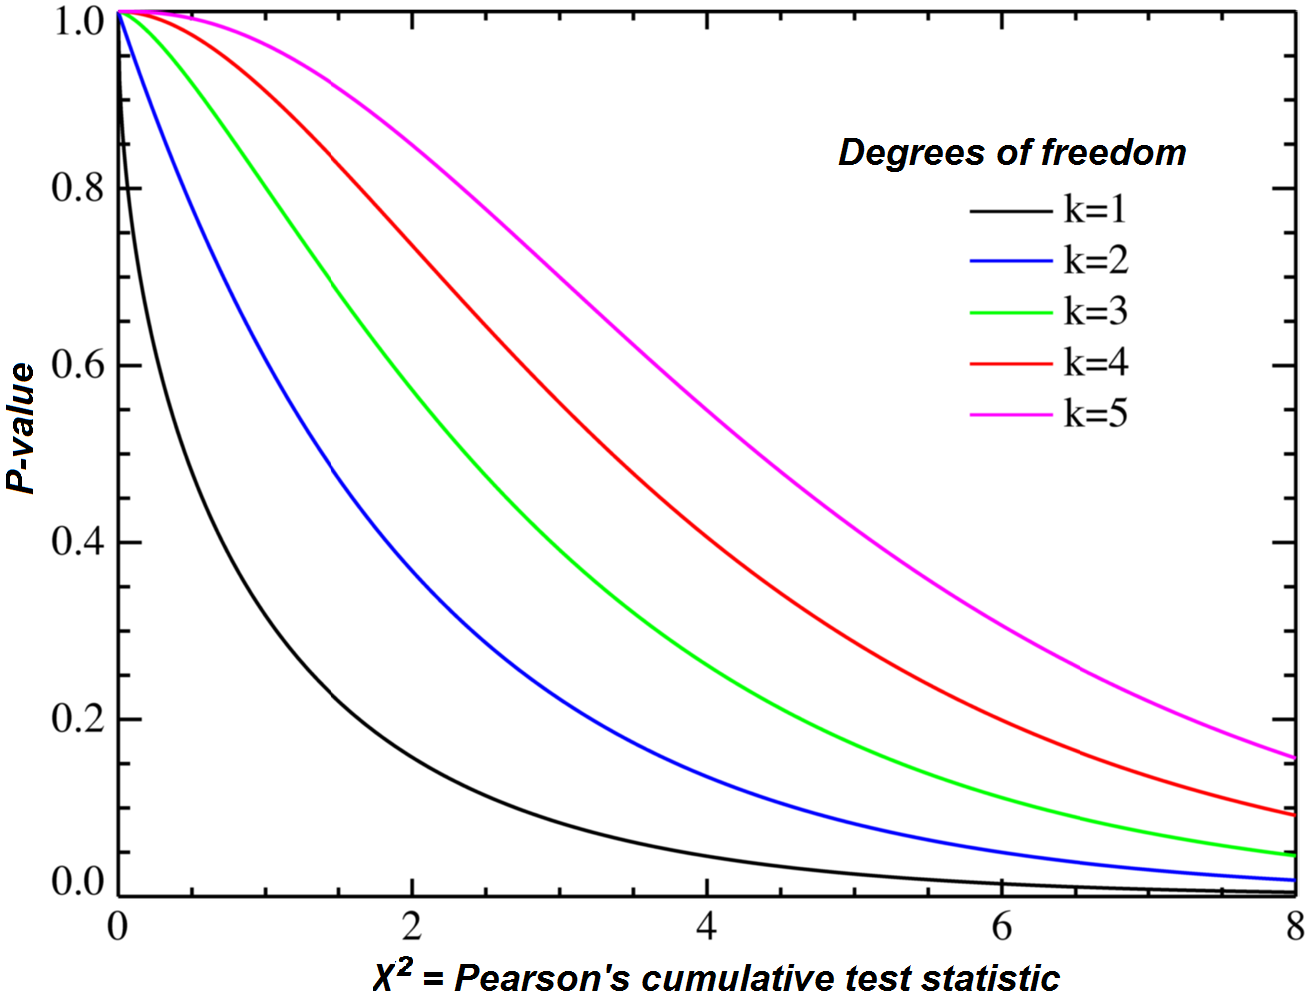
\includegraphics[scale=0.25]{pics/wk4/chi2.png}
\end{center}

Wikipedia
\end{frame}


\begin{frame}{Goodness of Fit in R}

\texttt{e <- predict(fit\_function, x)}\\
\texttt{chisq.test(y, p = e/sum(e))}

\end{frame}


\begin{frame}{Prediction}

``Prediction is hard, especially about the future.''

\end{frame}


\begin{frame}{Prediction Ranges}

Be careful\ldots

\vspace{5mm}

How to stay out of trouble:
\begin{itemize}
\item Don't make predictions
\item If you must make predictions, don't make them too far in the future
\item What is too far in the future?
\end{itemize}

\end{frame}



\begin{frame}{Now all the warnings are over\ldots}

Making predictions in R:
\begin{itemize}
\item Find a variable that can be used as a predictor for another (\texttt{plot()}, \texttt{pairs()}, \ldots)
\item Fit a suitable function (\texttt{lm()} or \texttt{nls()})
\item extrapolate that fit funtion and its errors (\texttt{predict()})
\end{itemize}

\end{frame}

\begin{frame}{Week 4 Problems}

\begin{enumerate}
\item Fitting Data
\item Making predictions
\end{enumerate}



\end{frame}




%%%%%%%%%%%%% backup slides %%%%%%%%%%%%%%%%%%%%%%%%

\appendix
\newcounter{finalframe}
\setcounter{finalframe}{\value{framenumber}}

\begin{frame}{Backup Slides}
\end{frame}




\setcounter{framenumber}{\value{finalframe}}

\end{document}
